\title{PDE Solver}
\date{}

\documentclass[12pt]{article}

\usepackage[italian]{babel}
\usepackage[T1]{fontenc}
\usepackage[utf8]{inputenc}
\usepackage{graphicx}
\usepackage{amsmath}
\usepackage{amssymb}
\usepackage{float}

\begin{document}
\maketitle
\newpage

\section{Introduzione}
La richiesta dell'\emph{assignment} è stata quella di implementare un semplice risolutore di equazioni differenziali alle derivate parziali con il \emph{metodo delle differenze finite}. Utilizzando la CPU, \emph{single core}, prima e la GPU, in seguito.

\subsection{Metodo delle differenze finite}
Il metodo delle differenze finite permette di valutare l'evoluzione a regime di un equazione differenziale alle derivate parziali, in due variabili nel caso preso in esame.

Si alloca una matrice di dimensione $(N+2) \times (N+2)$ e si impone la condizione al contorno sull'orlo della matrice, nel caso di studio, ogni elemento appartenente all'orlo della matrice è stato posto a $1.0$.

L'evoluzione all'iterazione \emph{n-esima} è data dalla seguente trasformazione applicata 
ad ogni elemento della matrice $ \phi \in \mathbb{R}^{N \times N}$ più interna:
$$ \phi(x,y)_{n+1} = 0.25\left[ \phi(x+1,y)_n +\phi(x-1,y)_n +\phi(x,y+1)_n +\phi(x,y-1)_n  \right] $$

Che si traduce nell'aggiornare ogni elemento con la media dei $4$ elementi adiacenti.

\begin{figure}[H]
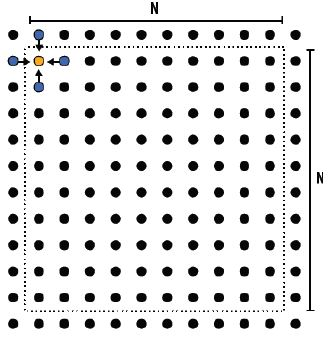
\includegraphics{PDE_normal.jpg}
\centering
\end{figure}


Per raggiungere lo stato di regime non è necessario evitare che nel calcolo vengano presi elementi dell'iterazione corrente già modificati in quanto il fenomeno, da un punto di vista non ha un ordine preferenziale.

\section{Parallelizzazione}
Al fine di parallelizzare l'algoritmo ed eseguirlo sulla GPU si è usato il metodo del \emph{Coloring}. Dividendo la matrice in celle rosse e nere, a onta di scacchiera, è possibile rendere indipendenti le due metà delle operazioni eseguite ad ogni iterazione.

\begin{figure}[H]
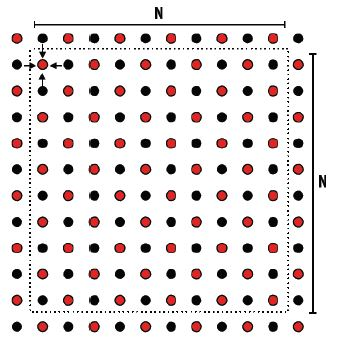
\includegraphics{PDE_coloring.jpg}
\centering
\end{figure}

Per l'implementazione in \emph{CUDA} si è scelto, per semplicità di dividere la matrice interna in blocchi da $ 512 \times 512 $ thread.

\section{Benchmark}
La complessità computazionale dell'algoritmo è quadratica rispetto a $N$, si nota infatti come il grafico dell'implementazione \emph{single thread} incrementi il tempo di esecuzione più che linearmente rispetto a $N$.

Per quanto riguarda l'implementazione GPU i tempi sono ridotti di 5 ordini di grandezza, nei test.

\begin{figure}[H]
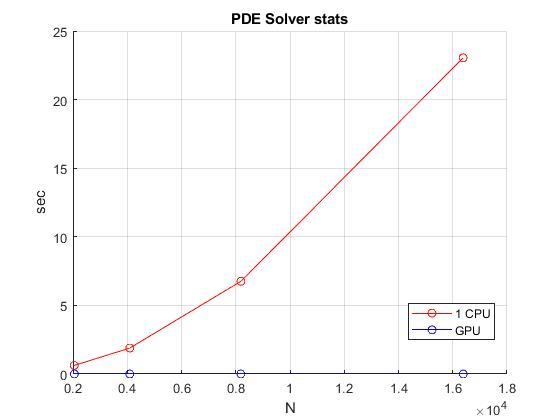
\includegraphics[width=\textwidth]{PDEStats.jpg}
\centering
\end{figure}


\section{Conclusioni}
Dal \emph{benchmark} è possibile notare come il problema sia altamente parallelizzabile e quanto la GPU si dimostri superiore per questo tipo di compito.

\end{document}
